\documentclass{standalone}
\usepackage{graphicx}	
\usepackage{amssymb, amsmath}
\usepackage{color}

\usepackage{tikz}
\usetikzlibrary{intersections, backgrounds, patterns, patterns.meta}
\usepackage{pgfmath}

\definecolor{light}{RGB}{220, 188, 188}
\definecolor{mid}{RGB}{185, 124, 124}
\definecolor{dark}{RGB}{143, 39, 39}
\definecolor{highlight}{RGB}{180, 31, 180}
\definecolor{gray10}{gray}{0.1}
\definecolor{gray20}{gray}{0.2}
\definecolor{gray30}{gray}{0.3}
\definecolor{gray40}{gray}{0.4}
\definecolor{gray60}{gray}{0.6}
\definecolor{gray70}{gray}{0.7}
\definecolor{gray80}{gray}{0.8}
\definecolor{gray90}{gray}{0.9}
\definecolor{gray95}{gray}{0.95}

\begin{document}

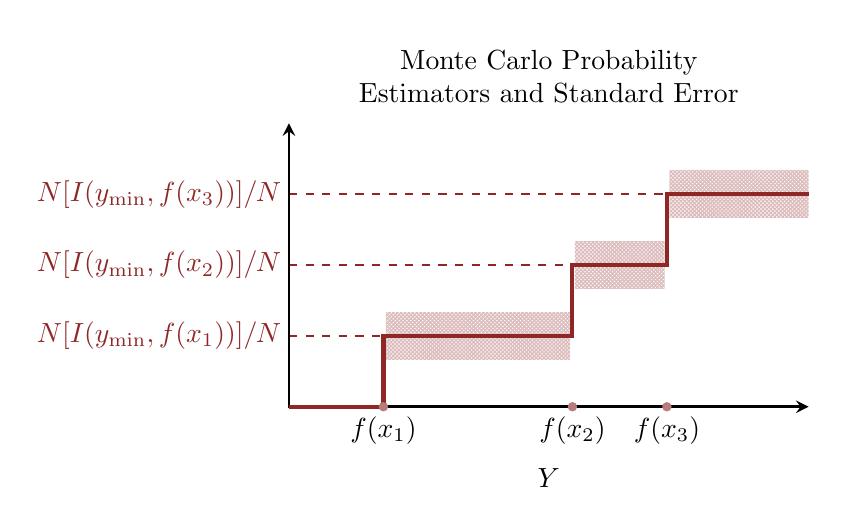
\begin{tikzpicture}[scale=0.3, thick]

\begin{scope}[shift={(0, 0)}]
  \draw[white] (-22, -4) rectangle (12, 16);
  \node[align=center] at (0, 14) { Monte Carlo Probability\\Estimators and Standard Error };

  \draw[dark, dashed] (-11, 3) -- (-7, 3);
  \node[dark] at (-16.5, 3) { $N[I(y_{\text{min}}, f(x_{1}))] / N$ };

  \draw[dark, dashed] (-11, 6) -- (1, 6);
  \node[dark] at (-16.5, 6) { $N[I(y_{\text{min}}, f(x_{2}))] / N$ };
  
  \draw[dark, dashed] (-11, 9) -- (5, 9);
  \node[dark] at (-16.5, 9) { $N[I(y_{\text{min}}, f(x_{3}))] / N$ };

  \draw [->, >=stealth, line width=1] (-11, 0) -- (-11, 12);

  \draw [->, >=stealth, line width=1] (-11.05, 0) -- (11, 0);
  \node at (0, -3) { $Y$ };
  
  \fill[pattern={Hatch[angle=45,distance=1, line width=0.5]}, pattern color=light] 
    (-7 + 0.1, 2) rectangle (1 - 0.1, 4);

  \fill[pattern={Hatch[angle=45,distance=1, line width=0.5]}, pattern color=light] 
    (1 + 0.1, 5) rectangle (5 - 0.1, 7);
    
  \fill[pattern={Hatch[angle=45,distance=1, line width=0.5]}, pattern color=light] 
    (5 + 0.1, 8) rectangle (11, 10);
  
  \draw[dark, line width=1.5] (-11, 0) -- (-7, 0) -- (-7, 3) -- (1, 3) -- (1, 6) -- (5, 6) -- (5, 9) -- (11, 9);
  
  \fill[mid] (-7, 0) circle (0.2);
  \node at (-7, -1) { $f(x_{1})$ };
  
  \fill[mid] (1, 0) circle (0.2);
  \node at (1, -1) { $f(x_{2})$ };
  
  \fill[mid] (5, 0) circle (0.2);
  \node at (5, -1) { $f(x_{3})$ };
  
\end{scope}
  
\end{tikzpicture}

\end{document}  